\documentclass{article}%
\usepackage[T1]{fontenc}%
\usepackage[utf8]{inputenc}%
\usepackage{lmodern}%
\usepackage{textcomp}%
\usepackage{lastpage}%
\usepackage[head=40pt,margin=0.5in,bottom=0.6in]{geometry}%
\usepackage{graphicx}%
%
\title{\textbf{Trabajadores del IND protestan para rechazar reducción de tabla salarial}}%
\author{El Nacional Web}%
\date{16/10/2018}%
%
\begin{document}%
\normalsize%
\maketitle%
\textbf{URL: }%
http://www.el{-}nacional.com/noticias/protestas/trabajadores{-}del{-}ind{-}protestan{-}para{-}rechazar{-}reduccion{-}tabla{-}salarial\_255945\newline%
%
\textbf{Periodico: }%
EN, %
ID: %
255945, %
Seccion: %
Protestas\newline%
%
\textbf{Palabras Claves: }%
NO\_TIENE\newline%
%
\textbf{Derecho: }%
2.3%
, Otros Derechos: %
NO\_TIENE%
, Sub Derechos: %
2.3.4%
\newline%
%
\textbf{EP: }%
SI\newline%
\newline%
%
\textbf{\textit{Los empleados indican que las~autoridades buscan contemplar bonificaciones y beneficios dentro del salario mínimo~}}%
\newline%
\newline%
%
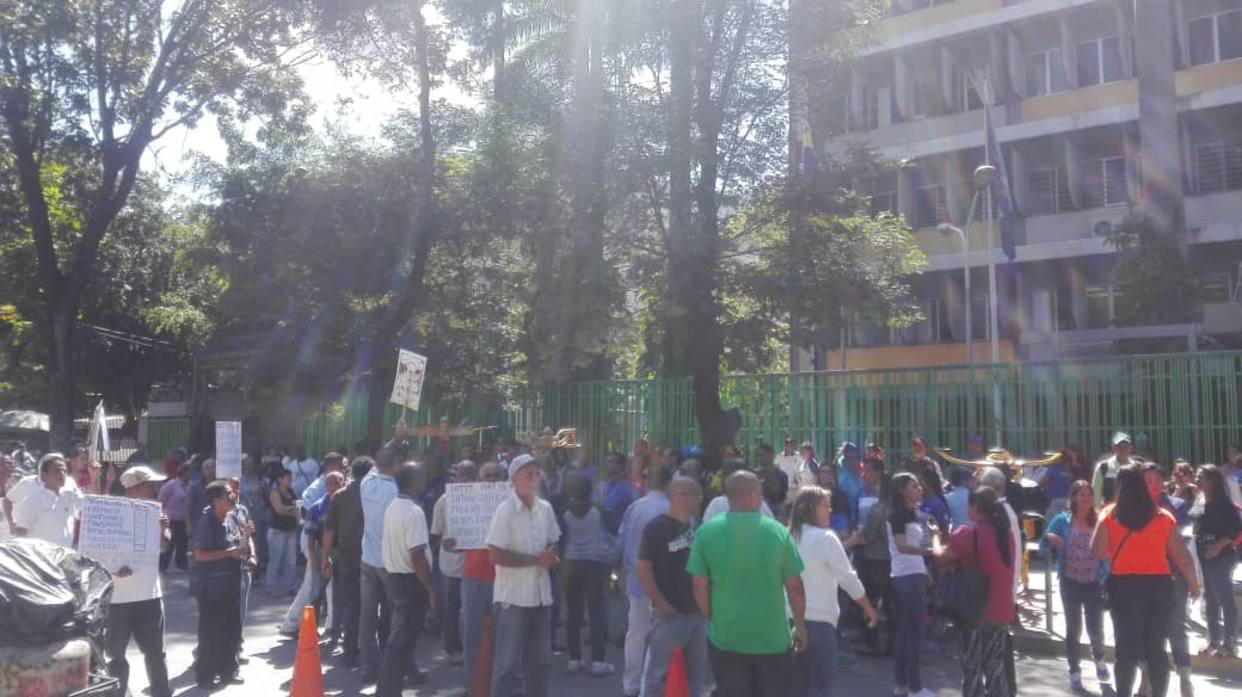
\includegraphics[width=300px]{60.jpg}%
\newline%
%
Trabajadores del Instituto de Deportes (IND) protestan este martes en la avenida intercomunal de Montalbán para rechazar la reducción la tabla salarial implementada por el gobierno.%
\newline%
%
Reportes de Twitter indican que desde las 10:40 am los empleados están en la calle. Manifiestan que las~autoridades buscan contemplar bonificaciones y beneficios dentro del salario mínimo BsS 1.800%
\newline%
%
Durante la mañana de hoy varios gremios salieron a las calles a exigir reivindicaciones salariales y respeto a los contratos colectivos.%
\newline%
%
\end{document}